% 兰姆位移

\pentry{玻尔原子模型\upref{BohrMd}}

\footnote{参考 HyperPhysics \href{http://hyperphysics.phy-astr.gsu.edu/hbase/quantum/lamb.html}{相关条目}.}根据狄拉克的量子理论, 氢原子的 $2S_{1/2}$ 和 $2P_{1/2}$ 能级应该具有相同的能量, 但兰姆的实验发现它们有微弱的偏差, 前者高出约
\begin{equation}
\Delta E = 4.372\times 10^{-6} \Si{eV}
\end{equation}
这被称为\textbf{兰姆位移(Lamb shift)}.

\autoref{LambSh_fig1} 中显示, $n=2$ 能级的精细结构由 $2P_{3/2}$ 和 $2P_{1/2}$ 构成, 而兰姆位移由 $2S_{1/2}$ 和 $2P_{1/2}$ 构成. 兰姆位移和氢原子基态的超精细结构\upref{HydroL}在同一个数量级. 
\begin{figure}[ht]
\centering
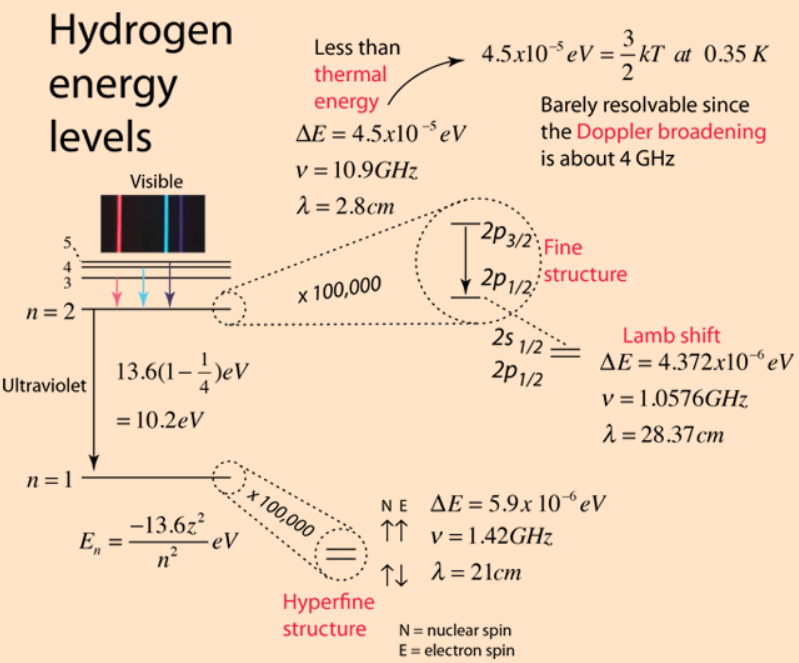
\includegraphics[width=12cm]{./figures/LambSh_1.png}
\caption{氢原子的精细结构, 超精细结构, 以及兰姆位移(来自 \href{http://hyperphysics.phy-astr.gsu.edu/hbase/quantum/lamb.html}{HyperPhysics})} \label{LambSh_fig1}
\end{figure} % 未完成: 图片侵权, 需要重画

\subsection{补充}
(未完成)Hans Bethe 首先用量子电动力学解释了兰姆位移.

(未完成)兰姆位移用于精确测量精细结构常数.

\subsection{能级修正}
事实上, 兰姆位移对每个能级都有微小的修正\footnote{详见 Bethe, H.A.; Salpeter, E.E. (1957). Quantum Mechanics of One- and Two-Electron Atoms. Springer. p. 103.}
\begin{equation}
\Delta E_{lamb} = \alpha^5 m_e c^2 \frac{k(n, 0)}{4n^3} \qquad (l = 0)
\end{equation}
\begin{equation}
\Delta E_{lamb} =\alpha^5 m_e c^2 \frac{1}{4n^3} \qty[k(n,l) \pm \frac{1}{\pi(j+1/2)(l+1/2)} ] \qquad (l \ne 0,\ j = l \pm 1/2)
\end{equation}
其中 $k(n, 0)$ 约等于 $13$, $k(n, l) < 0.05$ . 将 $2S_{1/2}$ ($l = 0$) 和 $2P_{1/2}$ ($n = 2,\ l = 1,\ s = 1/2$), 得 $\Delta E = 4.365\times 10^{-6}$.
